\section{Methods} \label{sec:methods}

In this section, we describe the primary two algorithmic components for our on-device simulation:
\begin{enumerate}
\item the asynchronous compute-communicate cycle used to instantiate an island model evolutionary process across the WSE engine, and
\item the lightweight hereditary stratigraphy element used to annotate virtual genomes and facilitate robust post-hoc phylogenetic reconstruction.
\end{enumerate}

\subsection{Asynchronous Island-model Evolutionary Computaiton}

We apply an island-model genetic algorithm to instantiate an evolutionary process spanning PEs.
Island-model approaches are common in applications of parallel and distributed computing to evolutionary computation \citep{kozaTODO}.
Under this model, each processor elemement (PE) hosts an independent population.
Migration between PEs stitches island populations together into a common gene pool.

\begin{figure}[htbp]
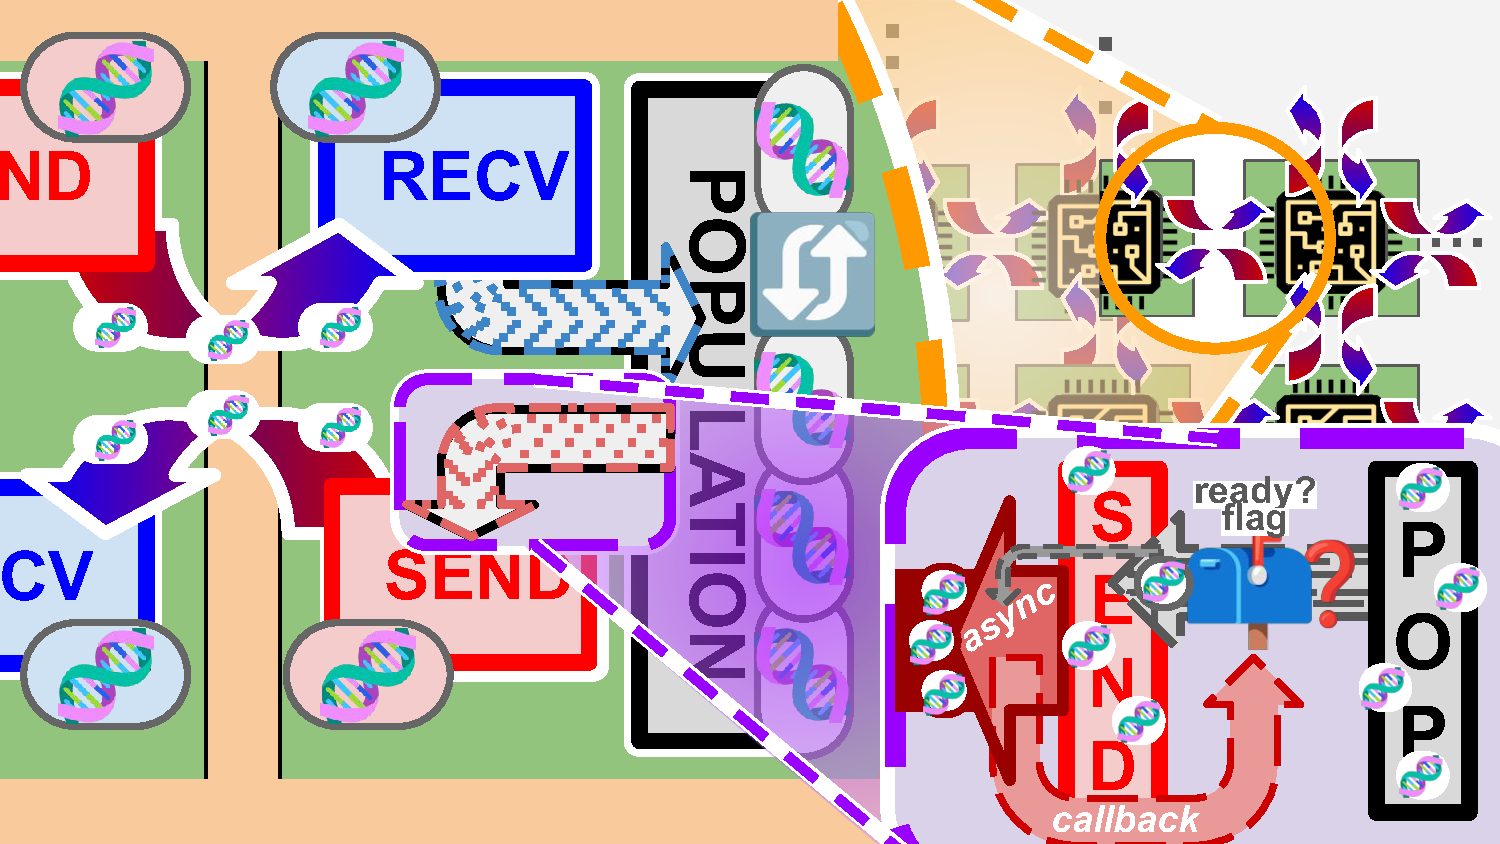
\includegraphics[width=4in]{img/async-ga-schematic.pdf}
\centering
\caption{Schematic overview of asynchronous island model evolutionary algorithm.}
\label{fig:async-ga-schematic}
\end{figure}

Core kernel activity proceeds via an update cycle performed on eacch PE, which comprises several steps.
Figure \ref{fig:async-ga-schematic} provides a schematic overview.

The first step of this update loop is to handle migration, depicted as blue-red arrows in Figure \ref{fig:async-ga-schematic}.
We adopt a fully asynchronous approach to migration between neighboring PEs.
Evolutionary processes tend to occur in asynchronous manner with arbitrary factors influencing things, so this is a reasonable relaxation to make.

Each PE maintains independent immigration buffers and emigration buffers dedicated to each cardinal neighbor, depicted in blue and red, respectively, in Figure \ref{fig:async-ga-schematic}.
On simulation startup, an asynchronous DSD receive operation is opened to accept genomes from neighboring PEs into the appropriate immigration buffer.
At startup, additionally, the emigration buffer is populated with one or more genomes copied the population.
Then, an asynchronous send request is opened to dispatch wavelets containing genome data from the emigration buffer to the neighbor.
Both operations register an on-completion callback to set a ``send complete'' or ``receive complete'' flag variable associated with their corresponding buffer.

Each update cycle, the the main update loop tests all ``send complete'' and ``receive complete'' flags.
For each immigration flag that is set, corresponding received genomes are written into the main population buffer, replacing randomly-chosen population members.
Then, the flag is reset a new receive request is initiated.
Likewise, for each emigration flag set, corresponding send buffers are re-populated with randomly sampled genomes from the main population buffer.
Corresponding flags are then reset and new send requests initiated.
The bottom right corner of Figure \ref{fig:async-ga-schematic} summarizes this process.

The remainder of the mmain update loop handles evolutionary operations witin the scope of the executing PE.
Each genome within the population is evaluated to produce a floating point fitness value.
Modular implementation ensures evaluation criteria can chosen appropriate for underlying experimental objectives.
For the purposes this project, we will use a trivial fitness function that explicitly models additive accumulation of beneficial/deleterious mutations as a floating point value within each genome.

After evaluation, tournament selection is applied.
Each slot in the next generaiton is populated with a genome exhibiting maximal fitness among $n$ randomly sampled individuals, ties broken randomly.

Finally, a mutational operator is applied across all genomes in the next population.
As with evaluation criteria, modular implementation allows mutation operations to be defined based on experimental objectives.
Here, we use a simple gaussian mutation on each genome's stored fitness value.
At this point, hereditary stratigraphy annotations --- discussed next --- are updated to reflect an elapsed generation.

The process then repeats, with self-activating wavelet dispatched to execute the next cycle of the main update loop.

Kernel source code implementing described procedures can be viewed at \url{https://hopth.ru/cl}.
Our implementation is defined modularly with respect to genome size, layout, mutational operator, and fitness evaluation criteria, allowing for direct re-use of produced software for follow-on evolution experiments on WSE hardware.

% A key question will be the extent to which intentionally desynchronizing affects performance, stability, and computation quality.

\subsection{Distributed Phylogenetic Tracking}

In pilot work with dynamically curated space-time memory buffers, we have achieved highly-scalable phylogenetic tracking in ABMS modelling of evolutionary processes \citep{morenoHstratPythonPackage2022, morenoHereditaryStratigraphyGenome2022}.
Our approach, hereditary stratigraphy (HStrat), uses a reconstruction-based strategy akin to how biologists build phylogenies.
Using heritable generational fingerprints, we achieve fast, accurate reconstruction.
To prevent $\mathcal{O}(n)$ space complexity, not all fingerprints can be kept.
Instead, we use a constant-time indexing scheme to map a stream of fingerprints onto a fixed-width memory buffer such that entries evicted by new placements maintain a temporally-representative sampling over elapsed time, either evenly (``steady'') or recency-biased (``tilted'') (Fig. \ref{fig:hstrat-schematic}).
Time stamps can be positionally inferred  --- a several-fold savings for small data objects. For example, single-bit checkpoints produce good quality phylogenies using only 12 bytes per genome \citep{moreno2023toward}.

It is necessary to optimize reconstruction to get high quality results with tractable genome sizes and limit the impact on memory usage and bandwidth usage.
Hereditary stratigraphy \citep{moreno2022hereditary} was designed to do this.

We have successfully demonstrated aspects of this approach (published in existing work as the hstrat Python library), with present work revising the underlying algorithms to better suit resource-constrained environments such as CS-2 Processor Elements.
Existing work targets traditional HPC environments \citep{moreno2022hstrat},
However, a highly compact, without advanced data structures is necessary to support the Cerebras WSE.
This led to development of unpublished variant of existing hereditary stratigraphy, the hereditary stratigraphic surface.

\begin{wrapfigure}{r}{0.5\textwidth}
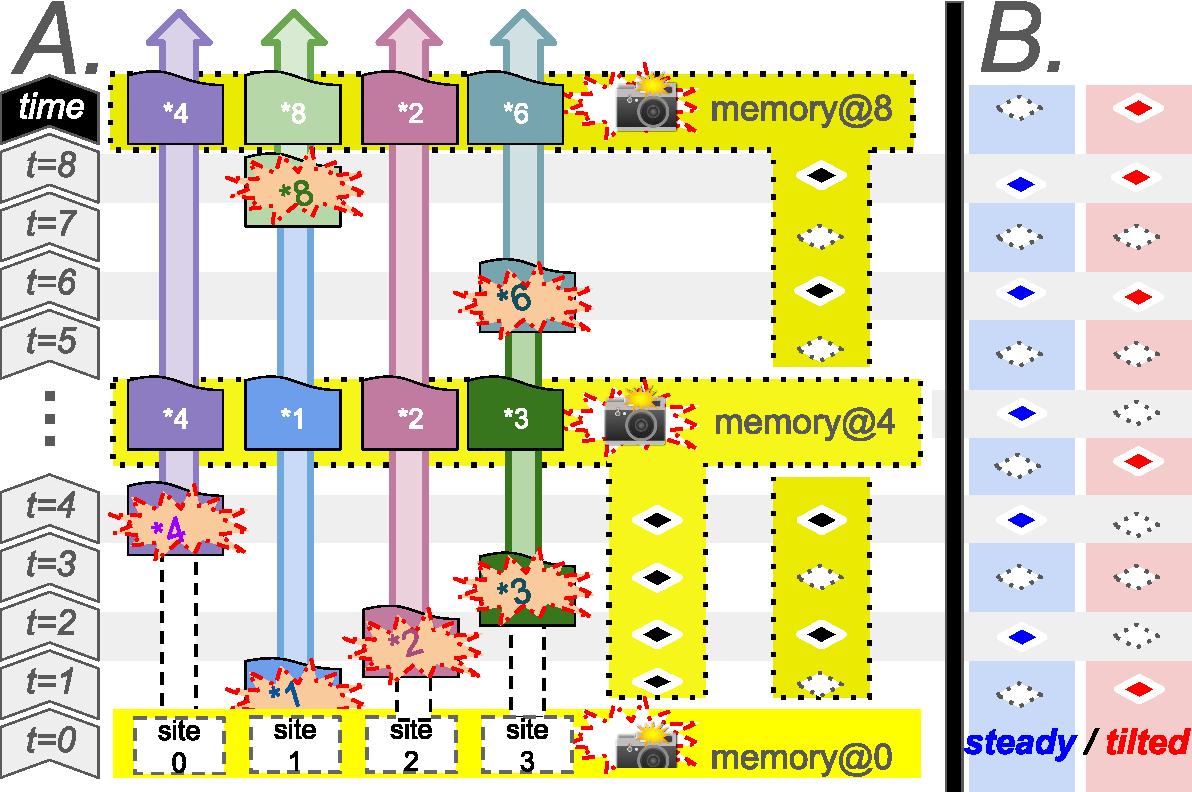
\includegraphics[width=\linewidth]{img/hsurf-schematic.pdf}
\centering
\caption{Panel A shows update sequence on a four-site HStrat curation space-time memory under steady policy. Panel B contrasts steady policy with tilted policy, which prioritizes recent data.}
\label{fig:hsurf-schematic}
\end{wrapfigure}


Instead of being maintained within a sorted list, lineage checkpoint markers are stored in a flat buffer.
This couples curation --- adding a checkpoint implicitly removes the checkpoint it overwrites.
The indexing scheme can be computed in $\mathcal{O(1)}$ time with respect to the size of the buffer and to the number of generaitons elapsed.

This genome has two components: a generation counter and the checkpoint marker buffer.
